\PassOptionsToPackage{hyphens}{url}
\documentclass[superscriptaddress, nofootinbib,  amsmath, amssymb, twocolumn]{revtex4-2} % twocolumn causing issues with neverending spillover into invisible area past first page

% \usepackage{balance}

% \usepackage[margin=1.5cm]{geometry} 
\usepackage[english]{babel}
\usepackage[utf8]{inputenc}
\usepackage[]{graphicx}
\usepackage{xspace}
\usepackage{siunitx}
\usepackage{mhchem}
\DeclareSIUnit\angstrom{\text {Å}}
\usepackage{orcidlink}
\usepackage{hyperref}
\usepackage{fontawesome5}
\usepackage{natmove}
\usepackage{placeins}

\usepackage{ifthen}        % For conditional statements


\usepackage{longtable}



% % Initialize a macro to keep track of seen project names
% \newcommand{\projectnamesseen}{}

% % Define a macro to select the appropriate social media icon
% \newcommand{\socialmediaicon}[1]{%
%     \IfSubStr{#1}{twitter.com}{\faTwitter}{%
%     \IfSubStr{#1}{linkedin.com}{\faLinkedin}{%
%     \IfSubStr{#1}{facebook.com}{\faFacebook}{%
%     \IfSubStr{#1}{instagram.com}{\faInstagram}{\faLink}}}}%
% }
% \DTLloadrawdb[keys={ProjectNum,ProjectLink,ProjectName,TeamName,FirstName,LastName,Email,Organization,Industry/Academia/Gov't,City,Address,GithubRepo,SocialMediaLink,VideoLink}]{stores}{test.csv}

\usepackage{xparse}
\usepackage[a-1b]{pdfx}
% \usepackage[allfiguresdraft]{draftfigure}

\usepackage[disable]{todonotes}
% \usepackage{todonotes}

\newcommand{\githublink}[2]{
  \href{https://github.com/#1/#2}{\faGithub\ \url{#1/#2}}
}

\newcommand{\twitterlink}[1]{
  \href{#1}{\faTwitter}
}

\newcommand{\zenodolink}[1]{
  \href{https://doi.org/#1}{\faArchive\ \url{#1}}
}

%https://twitter.com/SamCox822/status/1641484192566460416?s=20

\newcommand{\formatlinks}[3]{%
    \href{\ifx\empty#1\empty N/A\else#1\fi}{\faGithub}\,%
    \href{\ifx\empty#2\empty N/A\else#2\fi}{\faVideo}\,%
    \href{\ifx\empty#3\empty N/A\else#3\fi}{\faTwitter}  % Adjust the icon based on social media type
}


\newcommand{\hflogo}{%

\includegraphics[height=.9em]{figures/huggingface.png}
}

\newcommand{\huggingfacelink}[2]{
  \href{https://huggingface.co/spaces/#1/#2}{\hflogo \url{#1/#2}}
}

\newcommand{\huggingfacehublink}[2]{
  \href{https://huggingface.co/#1/#2}{\hflogo \url{#1/#2}}
}

% Adjusted Hyperref Setup for Automatically Colored Text Links
\hypersetup{
  colorlinks=true,       % Enables colored links
  breaklinks=true,
  urlcolor=blue,         % Sets the color of URL links
  linkcolor=blue,        % Sets the color of internal links
  citecolor=blue,        % Sets the color of citation links
  filecolor=blue,        % Sets the color of file links
  allcolors=blue,        % Ensures all link types are blue by default
  pdftitle={Title},      % PDF Title
  pdfauthor={Author}     % PDF Author
}

\usepackage[nameinlink,capitalise]{cleveref} %needs to appear after hyperref, https://tex.stackexchange.com/questions/396728/my-equations-referencing-not-working
\Crefname{figure}{Figure}{Figures} %needs to appear after hyperref and cleveref
\crefname{appsec}{Appendix}{Appendices}
\newcommand\crefrangeconjunction{--} % modify the reference style


% =====================================================
% packages for creating code listings 
\usepackage{listings, xcolor}
\definecolor{codegreen}{rgb}{0,0.6,0}
\definecolor{codegray}{rgb}{0.5,0.5,0.5}
\definecolor{codepurple}{rgb}{0.58,0,0.82}
\definecolor{tqblue}{HTML}{08293d}
\definecolor{backcolour}{HTML}{fefdf5}

\lstdefinestyle{pythonstyle}{
    backgroundcolor=\color{backcolour},   
    commentstyle=\color{codegreen},
    keywordstyle=\color{magenta},
    numberstyle=\tiny\color{codegray},
    stringstyle=\color{codepurple},
    basicstyle=\ttfamily\footnotesize\color{tqblue},
    breakatwhitespace=false,         
    breaklines=true,
    postbreak=\mbox{\textcolor{magenta}{$\hookrightarrow$}\space},                 
    captionpos=b,                    
    keepspaces=true,                 
    numbers=left,                    
    numbersep=5pt,                  
    showspaces=false,                
    showstringspaces=false,
    showtabs=false,                  
    tabsize=2
}

\lstset{style=pythonstyle}
\hbadness=99999 

\newcolumntype{C}{>{$}c<{$}}

\AtBeginDocument{%
  \heavyrulewidth=.08em
  \lightrulewidth=.05em
  \cmidrulewidth=.03em
  \belowrulesep=.65ex
  \belowbottomsep=0pt
  \aboverulesep=.4ex
  \abovetopsep=0pt
  \cmidrulesep=\doublerulesep
  \cmidrulekern=.5em
  \defaultaddspace=.5em
}



\usepackage[most]{tcolorbox}

\tcbset {
  base/.style={
    arc=0mm, 
    bottomtitle=0.5mm,
    boxrule=0mm,
    colbacktitle=black!10!white, 
    coltitle=black, 
    fonttitle=\bfseries, 
    left=2.5mm,
    leftrule=1mm,
    right=8.5mm,
    title={#1},
    toptitle=0.75mm, 
    width=\textwidth,
    breakable
  }
}

\definecolor{brandblue}{rgb}{0, 0.27843137254902, 0.466666666666667}
\newtcolorbox{agentinteraction}[1]{
  colframe=brandblue, 
  base={#1}
}


\definecolor{brandbred}{rgb}{0.63921568627451, 0, 0}
\newtcolorbox{agentinteraction2}[1]{
  colframe=brandbred, 
  base={#1}
}


\newtcolorbox{subbox}[1]{
  colframe=black!30!white,
  base={#1}
  }

\usepackage [autostyle, english = american]{csquotes}
\MakeOuterQuote{"}
\usepackage[acronym, nonumberlist]{glossaries}
\glsdisablehyper
\makeglossaries

\newacronym{llm}{LLM}{large language model}
\newacronym{gpt}{GPT}{generative pretrained transformer}
\newacronym{api}{API}{application programming interface}
\newacronym{ml}{ML}{machine learning}
\newacronym{lift}{LIFT}{language-interfaced fine-tuning}
\newacronym{icl}{ICL}{in-context learning}
\newacronym{peft}{PEFT}{parameter efficient fine-tuning}
\newacronym{lora}{LoRA}{low-rank adaptors}
\newacronym{gpr}{GPR}{Gaussian process regression}
\newacronym{ga}{GA}{genetic algorithm}
\newacronym{svm}{SVM}{support vector machine}
\newacronym{rf}{RF}{random forest}

\newacronym{ord}{ORD}{Open Reaction Database}
\newacronym{bo}{BO}{Bayesian optimization}
\newacronym{id}{ID}{inverse design}
\newacronym{mad}{MAD}{median absolute deviation}
\newacronym{eln}{ELN}{electronic lab notebook}
\newacronym[shortplural=LIMS]{lims}{LIMS}{laboratory information system}
\newacronym{ui}{UI}{user interface}
\newacronym{nlm}{NLM}{national library of medicine} 
\newacronym{dft}{DFT}{density functional theory}
\newacronym{cot}{COT}{chain of thought}
\newacronym{gui}{GUI}{graphical user interface}
\newacronym{pdb}{PDB}{protein data bank}
\newacronym{rlhf}{RLHF}{reinforcement learning from human feedback}
\newacronym{json}{JSON}{JavaScript object notation}
\newacronym{smiles}{SMILES}{simplified molecular-input line-entry system}
\newacronym{selfies}{SELFIES}{self-referencing embedded strings}
\newacronym{ai}{AI}{artificial intelligence}
\newacronym{nlp}{NLP}{natural language processing}
\newacronym{ner}{NER}{named entity recognition}
\newacronym{cas}{CAS}{Chemical Abstract Services}
\newacronym{mae}{MAE}{mean absolute error}
\newacronym{inchi}{InChI}{international chemical identifier}
\newacronym{mapi}{MAPI}{Materials Project \gls{api}}
\newacronym{rouge}{ROUGE}{Recall-Oriented Understudy for Gisting Evaluation}
\newacronym{html}{HTML}{HyperText Markup Language}
\newacronym{doi}{DOI}{digital object identifier}
\newacronym{ocr}{OCR}{optical character recognition}

\usepackage{tabularx} % For flexible tables with adjustable column widths
\usepackage{booktabs} % For better table lines (\toprule, \midrule, \bottomrule)
\usepackage{cleveref}

\let\originalcite\cite
\renewcommand{\cite}[1]{\unskip~\originalcite{#1}}

\usepackage{setspace}

% \clubpenalty=10000
% \widowpenalty=10000
% \displaywidowpenalty=10000
\usepackage{titlesec}

\titlespacing{\subsection}
    {0pt}{9pt}{6pt}

\usepackage{array}
\usepackage{ragged2e}
\usepackage{nicefrac}
\usepackage[caption=false]{subfig}

\newcolumntype{P}[1]{>{\raggedright\arraybackslash}p{#1}}

\begin{document}

\title{Bayesian Optimization Hackathon for Chemistry and Materials}

% %ToDo: add contributed equally indication for participants

\newcommand{\equalcont}{\thanks{These authors contributed equally}}

\author{Kevin~Maik~Jablonka~\orcidlink{0000-0003-4894-4660}}
\email{mail@kjablonka.com}
\affiliation{Laboratory of Molecular Simulation (LSMO), Institut des Sciences et Ing\'{e}nierie Chimiques, Ecole Polytechnique F\'{e}d\'{e}rale de Lausanne (EPFL), Sion, Valais, Switzerland.}

\author{Qianxiang Ai~\orcidlink{0000-0002-5487-2539}}
\equalcont
\affiliation{Department of Chemical Engineering, Massachusetts Institute of Technology, Cambridge, Massachusetts 02139, United States.}

%\email{qai@mit.edu}


\author{Alexander~Al-Feghali~\orcidlink{0009-0004-8377-7049}} 
\equalcont
%\email{alexander.al-feghali@mail.mcgill.ca}
\affiliation{Department of Chemistry, McGill University, Montreal, Quebec, Canada.}

\author{Shruti~Badhwar~\orcidlink{0000-0002-3167-5348}}
\equalcont
\affiliation{Reincarnate Inc.}  
%\email{shruti@reincarnateartificial.com}

\author{Joshua~D.~Bocarsly~\orcidlink{0000-0002-7523-152X}}
\equalcont
 \affiliation{Yusuf Hamied Department of Chemistry, University of Cambridge, Lensfield Road, Cambridge, CB2 1EW, United Kingdom.} 
 
%\email{jb2382@cam.ac.uk} 

\author{Andres~M~Bran~\orcidlink{0000-0002-4432-3667}}
\equalcont
\affiliation{Laboratory of Artificial Chemical Intelligence (LIAC), Institut des Sciences et Ing\'{e}nierie Chimiques, Ecole Polytechnique F\'{e}d\'{e}rale de Lausanne (EPFL), Lausanne, Switzerland.} 
\affiliation{National Centre of Competence in Research (NCCR) Catalysis, Ecole Polytechnique F\'{e}d\'{e}rale de Lausanne (EPFL), Lausanne, Switzerland.}


\author{Stefan~Bringuier~\orcidlink{0000-0001-6753-1437}}
\equalcont
\affiliation{Independent Researcher, San Diego, CA, United States.}
%\email{stefanbringuier@gmail.com}

\author{L.~Catherine~Brinson~\orcidlink{0000-0003-2551-1563}}
\equalcont
\affiliation{Mechanical Engineering and Materials Science, Duke University, United States.}
%\email{cate.brinson@duke.edu}



\author{Defne~Circi~\orcidlink{0000-0002-5761-0198}}
\equalcont
\affiliation{Mechanical Engineering and Materials Science, Duke University, United States.}
%\email{defne.circi@duke.edu}

\author{Sam~Cox~\orcidlink{0000-0002-4441-9327}}
\equalcont
\affiliation{Department of Chemical Engineering, University of Rochester, United States.}
%\email{swrig30@ur.rochester.edu}

\author{Wibe~A.~de~Jong~\orcidlink{0000-0002-7114-8315}} 
\equalcont
\affiliation{Applied Mathematics and Computational Research Division, Lawrence Berkeley National Laboratory, Berkeley, CA 94720, United States.
}

\author{Matthew~L.~Evans~\orcidlink{0000-0002-1182-9098}}
\equalcont
 \affiliation{Institut de la Matière Condensée et des Nanosciences (IMCN), UCLouvain, Chemin des Étoiles 8, Louvain-la-Neuve, 1348, Belgium.}
 \affiliation{Matgenix SRL, 185 Rue Armand Bury, 6534 Gozée, Belgium.}
 %\email{matthew.evans@uclouvain.be}

 \author{Nicolas~Gastellu~\orcidlink{0000-0002-4052-076X}}
 \equalcont
\affiliation{Department of Chemistry, McGill University, Montreal, Quebec, Canada.}
%\email{nicolas.gastellu@mail.mcgill.ca} 

\author{Jerome~Genzling~\orcidlink{0009-0007-4728-1478}} 
\equalcont
\affiliation{Department of Chemistry, McGill University, Montreal, Quebec, Canada.}
%\email{jerome.genzling@mail.mcgill.ca}

\author{Mar\'ia~Victoria~Gil~\orcidlink{0000-0002-2258-3011}}
\equalcont
\affiliation{Instituto de Ciencia y Tecnolog\'ia del Carbono (INCAR), CSIC, Francisco Pintado Fe 26, 33011 Oviedo, Spain.}
%\email{victoria.gil@incar.csic.es}

\author{Ankur~K.~Gupta~\orcidlink{0000-0002-3128-9535}}
\equalcont
\affiliation{Applied Mathematics and Computational Research Division, Lawrence Berkeley National Laboratory, Berkeley, CA 94720, United States.
}


\author{Alishba~Imran}
\equalcont
\affiliation{Computer Science, University of California, Berkeley, Berkeley CA 94704, United States.}

\author{Sabine~Kruschwitz~\orcidlink{0000-0002-6296-4417}}
\equalcont
\affiliation{Bundesanstalt für Materialforschung und -prüfung, Unter den Eichen 87, 12205 Berlin, Germany.}
%\email{Sabine.Kruschwitz@bam.de}

\author{Anne~Labarre~\orcidlink{0000-0003-4939-3928}}
\equalcont
\affiliation{Department of Chemistry, McGill University, Montreal, Quebec, Canada.}
 %\email{Anne.Labarre@mail.mcgill.ca}  

\author{Jakub~Lála~\orcidlink{0000-0002-5424-5260}}
\equalcont
\affiliation{Francis Crick Institute, 1 Midland Rd, London NW1 1AT, United Kingdom.}
%\email{jakublala@gmail.com}
 
\author{Tao~Liu~\orcidlink{0000-0002-1082-5570}}
\equalcont
\affiliation{Department of Chemistry, McGill University, Montreal, Quebec, Canada.}
 %\email{tao.liu7@mail.mcgill.ca} 

\author{Steven~Ma~\orcidlink{0000-0006-9448-7332}}
\equalcont
\affiliation{Department of Chemistry, McGill University, Montreal, Quebec, Canada.}
 %\email{Steven.Ma@mail.mcgill.ca} 

\author{Sauradeep~Majumdar~\orcidlink{0000-0002-2095-3082}}
\equalcont
\affiliation{Laboratory of Molecular Simulation (LSMO), Institut des Sciences et Ing\'{e}nierie Chimiques, Ecole Polytechnique F\'{e}d\'{e}rale de Lausanne (EPFL), Sion, Valais, Switzerland.}
%\email{sauradeep.majumdar@epfl.ch}

\author{Garrett~W.~Merz~\orcidlink{0000-0003-4737-3931}}
\equalcont
\affiliation{American Family Insurance Data Science Institute, University of Wisconsin-Madison, Madison WI 53706, United States.}


\author{Nicolas~Moitessier~\orcidlink{0000-0001-6933-2079}}
\equalcont
\affiliation{Department of Chemistry, McGill University, Montreal, Quebec, Canada.}
%;  Department of Chemistry, McGill University, Montreal, Quebec, Canada; orcid.org/; 
%\email{nicolas.moitessier@mcgill.ca}

\author{Elias~Moubarak~\orcidlink{0000-0001-8271-6800}}
\equalcont
\affiliation{Laboratory of Molecular Simulation (LSMO), Institut des Sciences et Ing\'{e}nierie Chimiques, Ecole Polytechnique F\'{e}d\'{e}rale de Lausanne (EPFL), Sion, Valais, Switzerland.}
%\email{elias.moubarak@epfl.ch}



\author{Beatriz~Mouriño~\orcidlink{0000-0003-1670-3985}}
\equalcont
\affiliation{Laboratory of Molecular Simulation (LSMO), Institut des Sciences et Ing\'{e}nierie Chimiques, Ecole Polytechnique F\'{e}d\'{e}rale de Lausanne (EPFL), Sion, Valais, Switzerland.}
%\email{beatriz.buenomourino@epfl.ch}

\author{Brenden~Pelkie~\orcidlink{0000-0001-7638-6366}}
\equalcont
\affiliation{Department of Chemical Engineering, University of Washington, Seattle, WA 98105, United States.} 
%\email{bgpelkie@uw.edu} 

\author{Michael~Pieler~\orcidlink{0000-0001-9186-7045}}
\equalcont
\affiliation{OpenBioML.org}
\affiliation{Stability.AI}
%\email{ michael.pieler@gmail.com}

\author{Mayk~Caldas~Ramos~\orcidlink{0000-0001-5336-2847}}
\equalcont
\affiliation{Department of Chemical Engineering, University of Rochester, United States.}
%\email{mcaldasr@ur.rochester.edu}

\author{Bojana~Ranković~\orcidlink{0000-0002-1476-6686}}
\equalcont
\affiliation{Laboratory of Artificial Chemical Intelligence (LIAC), Institut des Sciences et Ing\'{e}nierie Chimiques, Ecole Polytechnique F\'{e}d\'{e}rale de Lausanne (EPFL), Lausanne, Switzerland.}
\affiliation{National Centre of Competence in Research (NCCR) Catalysis, Ecole Polytechnique F\'{e}d\'{e}rale de Lausanne (EPFL), Lausanne, Switzerland.}


\author{Jacob~N.~Sanders~\orcidlink{0000-0002-2196-4234}}
\equalcont
\affiliation{Department of Chemistry and Biochemistry, University of California, Los Angeles, CA 90095, United States.}
%\email{jacosand@gmail.com}




\author{Philippe~Schwaller~\orcidlink{0000-0003-3046-6576}}
\equalcont
\affiliation{Laboratory of Artificial Chemical Intelligence (LIAC), Institut des Sciences et Ing\'{e}nierie Chimiques, Ecole Polytechnique F\'{e}d\'{e}rale de Lausanne (EPFL), Lausanne, Switzerland.}
\affiliation{National Centre of Competence in Research (NCCR) Catalysis, Ecole Polytechnique F\'{e}d\'{e}rale de Lausanne (EPFL), Lausanne, Switzerland.}

 
\author{Marcus~Schwarting}
\equalcont
 \affiliation{Department of Computer Science, University of Chicago, Chicago IL 60490, United States.}
 %\email{meschw04@uchicago.edu}


\author{Jiale~Shi~\orcidlink{0000-0002-5447-3925}}
\equalcont
\affiliation{Department of Chemical Engineering, Massachusetts Institute of Technology, Cambridge, Massachusetts 02139, United States.}
 %\email{jialele@mit.edu}
 
 \author{Berend~Smit~\orcidlink{0000-0003-4653-8562}}
%\email{berend.smit@epfl.ch}
\equalcont
\affiliation{Laboratory of Molecular Simulation (LSMO), Institut des Sciences et Ing\'{e}nierie Chimiques, Ecole Polytechnique F\'{e}d\'{e}rale de Lausanne (EPFL), Sion, Valais, Switzerland.}

\author{Ben~E.~Smith~\orcidlink{0000-0001-9673-2449}}
\equalcont
 \affiliation{Yusuf Hamied Department of Chemistry, University of Cambridge, Lensfield Road, Cambridge, CB2 1EW, United Kingdom.} 
%\email{bs542@cam.ac.uk} 


\author{Joren~Van~Herck~\orcidlink{009-0005-5108-5061}}
\equalcont
\affiliation{Laboratory of Molecular Simulation (LSMO), Institut des Sciences et Ing\'{e}nierie Chimiques, Ecole Polytechnique F\'{e}d\'{e}rale de Lausanne (EPFL), Sion, Valais, Switzerland.}
%\email{joren.vanherck@epfl.ch}


\author{Sean~Warren~\orcidlink{0000-0002-3670-0354}}
\equalcont
%\affiliation{}
%\email{sean.warren@gatech.edu}



\author{Sylvester~Zhang}
\equalcont
\affiliation{Department of Chemistry, McGill University, Montreal, Quebec, Canada.}

\author{Xiaoqi~Zhang\orcidlink{0000-0002-6507-6490}}
\equalcont
\affiliation{Laboratory of Molecular Simulation (LSMO), Institut des Sciences et Ing\'{e}nierie Chimiques, Ecole Polytechnique F\'{e}d\'{e}rale de Lausanne (EPFL), Sion, Valais, Switzerland.}
%\email{xiaoqi.zhang@epfl.ch}


\author{Ghezal~Ahmad~Zia~\orcidlink{0000-0002-9082-9423}} 
\equalcont
\affiliation{Bundesanstalt für Materialforschung und -prüfung, Unter den Eichen 87, 12205 Berlin, Germany.}
%\email{Ghezal-Ahmad.Zia@bam.de} 



% organiziers 

\author{KJ~Schmidt}
%\email{kj.schmidt913@gmail.com}
\affiliation{Globus, University of Chicago, Data Science and Learning Division, Argonne National Lab, United States.}

\author{Ian~Foster~\orcidlink{0000-0003-2129-5269}}
\affiliation{Department of Computer Science, University of Chicago, Data Science and Learning Division, Argonne National Lab, United States.}

\author{Ben~Blaiszik~\orcidlink{0000-0002-5326-4902}}
\email{blaiszik@uchicago.edu}
\affiliation{Globus, University of Chicago, Data Science and Learning Division, Argonne National Lab, United States.}




\author{Sterling~G.~Baird}
\author{Mehrad~Ansari}
\affiliation{Acceleration Consortium, 700 University Ave.\ Suite 1001, Toronto, ON M5G 1X6}

% one footnote, shared by both authors
\email[Corresponding authors: ]{\{sterling.baird,\,mehrad.ansari\}@utoronto.ca}

\author{Zartashia ~Afzal}
% \email{chemistzartashiaafzal@gmail.com}
\affiliation{ICodeGuru, Canal Road, Quaid-i-Azam Campus, Lahore, Punjab, Pakistan.}

\author{Qianxiang~Ai}
% \email{qai@mit.edu}
\affiliation{Massachusetts Institute of Technology, Massachusetts Institute of Technology, 77 Massachusetts Ave, Cambridge, MA 02139, United States.}

\author{Alexander~Al-Feghali}
% \email{alexander.al-feghali@mail.mcgill.ca}
\affiliation{McGill University, Canada, 845 Rue Sherbrooke O, Montréal, QC H3A 0G4.}

\author{Mathieu~Alain}
% \email{mathieu.alain.21@ucl.ac.uk}
\affiliation{University College London, Gower Street, London WC1E 6BT.}

\author{Roozbeh~Alishahian}
% \email{rooz.alishahian@mail.utoronto.ca}
\affiliation{University of Toronto, 27 King's College Circle, Toronto, ON M5S 1A1, Canada.}

\author{Matias~Altamirano}
% \email{matias.altamirano.22@ucl.ac.uk}
\affiliation{University College London, Gower Street, London WC1E 6BT.}

\author{Thomas~Andrews}
% \email{tsandrews@student.unimelb.edu.au}
\affiliation{University of Melbourne, CSIRO, Parkville VIC 3052.}

\author{Andy Sode~Anker}
% \email{ansoan@dtu.dk}
\affiliation{Technical University of Copenhagen and Oxford University, Anker Engelunds Vej 411, 2800 Kongens Lyngby, Danmark \& Mansfield Rd, Oxford OX1 3TA, United Kingdom.}

\author{Rija~Ansari}
% \email{rija.ansari@nrc-cnrc.gc.ca}
\affiliation{National Research Council of Canada, 1200 Montreal Road, Ottawa ON, K1A 0R6.}

\author{Samuel Ampofo~Appiah}
\affiliation{Ghana National Gas Company, Ghana National Gas Company, Gas House, 7th Avenue, Ridge West, Accra, Ghana.}

\author{Raul~Astudillo}
% \email{rastudil@caltech.edu}
\affiliation{California Institute of Technology, 315 Annenberg IST Center, 330 S Chester Ave, Pasadena, CA 91125, United States.}

\author{Ruhana~Azam}
% \email{ruhana@stanford.edu}
\affiliation{Stanford University, 353 Jane Stanford Way, Stanford, CA, 94305.}

\author{Mohammed~Azzouzi}
% \email{mohammed.azzouzi15@imperial.ac.uk}
\affiliation{Imperial College London, Exhibition Rd, South Kensington, London SW7 2AZ.}

\author{Suneel Kumar~BVS}
% \email{Suneelkumar.bvs@gmail.com}
\affiliation{Atomicas AI solutions private limited}

\author{Ben~Blaiszik}
% \email{blaiszik@uchicago.edu}
\affiliation{University of Chicago, 9700 S. Cass Avenue, Lemont, IL, USA.}

\author{Anna~Borisova}
% \email{anna.borisova@epfl.ch}
\affiliation{EPFL, Station 06, CH-1015 Lausanne, Switzerland.}

\author{Andres~Bran}
% \email{andres.marulandabran@epfl.ch}
\affiliation{EPFL, NCCR Catalysis, Station 06, CH-1015 Lausanne, Switzerland.}

\author{Darby~Brown}
\affiliation{EMD Electronics, Frankfurter Str. 250, 64293 Darmstadt, Germany.}

\author{Pengfei~Cai}
% \email{pengfeic@mit.edu}
\affiliation{Massachusetts Institute of Technology, 77 Massachusetts Avenue Cambridge, MA 02139.}

\author{Ting-Yeh~Chen}
% \email{chen.11026@buckeyemail.osu.edu}
\affiliation{The Ohio State University, 281 W Lane Ave, Columbus, OH 43210.}

\author{Curtis~Chong}
% \email{curtischong5@gmail.com}
% \affiliation{nan, nan.}

\author{Samantha~Corapi}
% \email{s.corapi@mail.utoronto.ca}
\affiliation{University Of Toronto, 27 King's College Circle, Toronto, ON M5S 1A1, Canada.}

\author{Mark~Croxall}
\affiliation{University of Toronto, 27 King's College Cir, Toronto, ON M5S 1A1.}

\author{Gbetondji~Dovonon}
% \email{gbetondji@matterhorn.studio}
\affiliation{University College London, Gower Street, London WC1E 6BT.}

\author{Jose Manuel Napoles~Duarte}

\author{Andrew~Falkowski}
% \email{andrew.falkowski@utah.edu}
\affiliation{University of Utah, University of Utah, 201 Presidents Circle, Salt Lake City, UT 84112, United States.}

\author{Giuseppe~Fisicaro}
% \email{giuseppe.fisicaro@imm.cnr.it}
\affiliation{Institute for Microelectronics and Microsystems (IMM), National Research Council (CNR), Institute for Microelectronics and Microsystems (IMM), National Research Council (CNR), Via del Fosso del Cavaliere 100, 00133 Rome, Italy.}

\author{Martin~Fitzner}
% \email{martin.fitzner@merckgroup.com}
\affiliation{Merck KGaA, Darmstadt, Germany, Frankfurter Straße 250, 64293 Darmstadt, Germany.}

\author{Quinn~Gallagher}
% \email{qg1361@princeton.edu}
\affiliation{Princeton University, Department of Chemical and Biological Engineering, Princeton University, Princeton, New Jersey 08540.}

\author{Sabah~Gaznaghi}
% \email{s.gaznaghi@uq.edu.au}
\affiliation{University of Queensland, Building 75, Cooper Rd, St Lucia QLD 4067, Australia.}

\author{Jérôme~Genzling}
% \email{jerome.genzling@mail.mcgill.ca}
\affiliation{McGill University, 845 Rue Sherbrooke O, Montréal, QC H3A 0G4.}

\author{Christoph~Griehl}
% \email{griehl@mpi-magdeburg.mpg.de}
\affiliation{Max Planck Institute for Dynamics of Complex Technical Systems , Sandtorstraße 1, 39112 Magdeburg, Germany.}

\author{Ryan-Rhys~Griffiths}
% \email{ryangriff123@gmail.com}
\affiliation{FutureHouse, 1405 Minnesota St, San Francisco, CA 94107.}

\author{Taicheng~Guo}
% \email{tguo2@nd.edu}
\affiliation{University of Notre Dame, Holy Cross Dr, Notre Dame, IN 46556.}

\author{Kehan~Guo}
% \email{kguo2@nd.edu}
\affiliation{University of Notre Dame, Holy Cross Dr, Notre Dame, IN 46556.}

\author{Nipun~Gupta}
% \email{nipun.gupta@utoronto.ca}
\affiliation{Acceleration Consortium, 700 University Ave suite 1001, Toronto, ON M5G 1X6.}

\author{Ankur~Gupta}
% \email{ankur@lbl.gov}
\affiliation{Lawrence Berkeley National Laboratory, 1 Cyclotron Rd, Berkeley, CA 94720.}

\author{Mohammad~Haddadnia}

\affiliation{University Of Harvard, Harvard University, Massachusetts Hall, Cambridge, MA 02138, United States.}

\author{Yuyang~Han}
% \email{yuyanghan@g.ucla.edu}
\affiliation{University of California, Los Angeles, 607 Charles E Young Dr E, Los Angles, CA 90093.}

\author{Karim Ben~Hicham}
\affiliation{RWTH Aachen, Templergraben 55, 52062 Aachen, Germany.}

\author{Joscha~Hoche}
% \email{joscha.hoche@merckgroup.com}
\affiliation{Merck KGaA, Darmstadt, Germany, Frankfurter Straße 250, 64293 Darmstadt, Germany.}

\author{Alexander V.~Hopp}
% \email{alexander.hopp@merckgroup.com}
\affiliation{Merck KGaA, Darmstadt, Germany, Frankfurter Straße 250, 64293 Darmstadt, Germany.}

\author{Marko~Huang}
% \email{marko.huang@mail.utoronto.ca}
\affiliation{Department of Chemistry, University of Toronto, Lash Miller Chemical Laboratories, 80 St.George Street.}

\author{Ayodeji~Ijishakin}
% \email{ayoijish@outlook.com}
\affiliation{University College London, Gower Street, London WC1E 6BT.}

\author{Ramsey~Issa}
% \email{ramseyissa@gmail.com}
\affiliation{University of Utah, University of Utah, 201 Presidents Circle, Salt Lake City, UT 84112, United States.}

\author{Yeonghun~Kang}
% \email{dudgns1675@kaist.ac.kr}
\affiliation{KAIST, KAIST (Korea Advanced Institute of Science and Technology), 291 Daehak-ro, Yuseong-gu, Daejeon 34141, South Korea.}

\author{Jungtaek~Kim}
% \email{jungtaek.kim.mail@gmail.com}
\affiliation{University of Pittsburgh, 3700 O'Hara St, Pittsburgh, PA 15261, United States.}

\author{Akshay~Kudva}
% \email{kudva.7@buckeyemail.osu.edu}
\affiliation{The Ohio State University, 281 W Lane Ave, Columbus, OH 43210.}

\author{Rubén~Laplaza}
% \affiliation{nan, nan.}

\author{Magdalena~Lederbauer}
% \email{mlederbauer@ethz.ch}
\affiliation{ETH Zurich, EPFL, Station 06, CH-1015 Lausanne, Switzerland.}

\author{Shi Xuan~Leong}
% \email{shixuan.leong@utoronto.ca}
\affiliation{Department of Chemistry, University of Toronto, Lash Miller Chemical Laboratories, 80 St.George Street.}

\author{Paul W.~Leu}
% \email{pleu@pitt.edu}
\affiliation{University of Pittsburgh, 3700 O'Hara St, Pittsburgh, PA 15261, United States.}

\author{Viola Muning~Li}
% \email{viola.muning-li@external.merckgroup.com}
\affiliation{Merck KGaA, Darmstadt, Germany, Frankfurter Straße 250, 64293 Darmstadt, Germany.}

\author{Mingxuan~Li}
% \email{mil152@pitt.edu }
\affiliation{University of Pittsburgh, 3700 O'Hara St, Pittsburgh, PA 15261, United States.}

\author{Tao~Liu}
% \email{tao.liu7@mail.mcgill.ca}
\affiliation{McGill University, Canada, 845 Rue Sherbrooke O, Montréal, QC H3A 0G4.}

\author{Stanley~Lo}
% \email{stanley.lo@mail.utoronto.ca}
\affiliation{University of Toronto, 27 King's College Circle, Toronto, ON M5S 1A1, Canada.}

\author{Jakub~Lála}
% \email{jl24018@ic.ac.uk}
\affiliation{Imperial College London, Exhibition Rd, South Kensington, London SW7 2AZ, United Kingdom.}

\author{Osman~Mamun}
% \email{mamun.che06@gmail.com}
% \affiliation{nan, nan.}

\author{Joseph~Manning}
\affiliation{University of Manchester, Oxford Rd, Manchester M13 9PL, United Kingdom.}

\author{Owen~Melville}
% \email{owen.melville@utoronto.ca}
\affiliation{Acceleration Consortium, 700 University Ave suite 1001, Toronto, ON M5G 1X6.}

\author{Michail~Mitsakis}
% \email{mitsakismichail@gmail.com}
\affiliation{Technical University of Denmark (DTU), Argous 64 \& Potamou 77, Kifissia, Athens, Greece.}

\author{Cameron~Movassaghi}
% \email{csmova@g.ucla.edu}
\affiliation{University of California, Los Angeles, 607 Charles E Young Dr E, Los Angles, CA 90093.}

\author{Madhav Reddy~Muthyala}
% \email{muthyala.7@buckeyemail.osu.edu}
\affiliation{The Ohio State University, 281 W Lane Ave, Columbus, OH 43210.}

\author{Marcel~Müller}
% \email{marcel.mueller@thch.uni-bonn.de}
\affiliation{Merck KGaA, Darmstadt, Germany / University of Bonn, Frankfurter Straße 250, 64293 Darmstadt, Germany.}

\author{Bozhao~Nan}
% \email{bnan@nd.edu}
\affiliation{University of Notre Dame, Holy Cross Dr, Notre Dame, IN 46556.}

\author{Vijay~Narasimhan}
\affiliation{EMD Electronics, Frankfurter Str. 250, 64293 Darmstadt, Germany.}

\author{Duc~Nguyen}
% \email{nqduc@stanford.edu}
\affiliation{Stanford University, 353 Jane Stanford Way, Stanford, CA, 94305.}

\author{Daniele~Ongari}
% \email{daniele.ongari@syensqo.com}
\affiliation{Syensqo , Viale Lombardia 20, Bollate, Italy.}

\author{Anthony~Onwuli}
% \email{anthony.onwuli16@imperial.ac.uk}
\affiliation{Imperial College London, Imperial College London, Exhibition Road, South Kensington, London SW7 2BX, United Kingdom.}

\author{Can~Özkan}
% \email{c.ozkan@tudelft.nl}
\affiliation{TU Delft, Mekelweg 5, 2628CD Delft, the Netherlands.}

\author{Sergio~Pablo-Garcia}
% \email{sp.garcia@utoronto.ca}
\affiliation{University of Toronto, Department of Chemistry, University of Toronto, Lash Miller Chemical Laboratories, 80 St.George Street.}

\author{Elton~Pan}
% \email{eltonpan@mit.edu}
\affiliation{Massachusetts Institute of Technology, 77 Massachusetts Avenue Cambridge, MA 02139.}

\author{Ratish~Panda}
% \email{ratishp2001@gmail.com}
\affiliation{Birla Institute of Technology, Mesra, Jharkhand 835215, India.}

\author{Sean~Park}
% \email{seanhs.park@mail.utoronto.ca}
\affiliation{University Of Toronto, University of Toronto, 27 King's College Circle, Toronto, ON M5S 1A1, Canada.}

\author{Jaehee~Park}
% \email{jaeheepark@uchicago.edu}
\affiliation{University of Chicago, 5801 S Ellis Ave, Chicago, IL 60637.}

\author{Brenden~Pelkie}
% \email{bgpelkie@uw.edu}
\affiliation{University of Washington, 3819 Okanogan Lane NE, Seattle, WA, 98195, USA.}

\author{Dieter~Plessers}
% \email{dieter.plessers@kuleuven.be}
\affiliation{KU Leuven, Celestijnenlaan 200F, 3001 Leuven, Belgium.}

\author{Tobias~Plötz}
% \email{tobias.ploetz@merckgroup.com}
\affiliation{Merck KGaA, Darmstadt, Germany, Frankfurter Straße 250, 64293 Darmstadt, Germany.}

\author{Utkarsh~Pratiush}
% \email{upratius@vols.utk.edu}
\affiliation{University of Tennessee, Knoxville, TN 37996, United States.}

\author{Ella M.~Rajaonson}
% \email{ella.rajaonson@mail.utoronto.ca}
\affiliation{University Of Toronto, University of Toronto, 27 King's College Circle, Toronto, ON M5S 1A1, Canada.}

\author{Bojana~Ranković}
% \email{bojana.rankovic@epfl.ch}
\affiliation{EPFL, NCCR Catalysis, Station 06, CH-1015 Lausanne, Switzerland.}

\author{Jarett~Ren}
% \email{jren25@jhu.edu}
\affiliation{Johns Hopkins University, 3400 N. Charles Street, Baltimore, MD 21218.}

\author{Rim~Rihana}
% \email{rim.rihana@merckgroup.com}
\affiliation{Merck KGaA, Darmstadt, Germany, Frankfurter Straße 250, 64293 Darmstadt, Germany.}

\author{Jurgis~Ruza}
% \email{jruza@mit.edu}
\affiliation{Massachusetts Institute of Technology, 77 Massachusetts Avenue Cambridge, MA 02139.}

\author{Akhil~S. Nair}
% \email{nair@fhi-berlin.mpg.de}
\affiliation{Fritz-Haber Institute of the Max-Planck Society,  Faradayweg 4-6, D-14195 Berlin, Germany.}

\author{Carter~Salbego}
% \email{carter.w.salbego@gmail.com}
\affiliation{University of Utah, University of Utah, 201 Presidents Circle, Salt Lake City, UT 84112, United States.}

\author{Erick Lopez~Saldivar}

\affiliation{Autonomous University of Chihuahua, Autonomous University of Chihuahua, Av. Escorza 900, Colonia Centro, 31000 Chihuahua, Chih., Mexico.}

\author{Arifin~San}
% \email{fin_ari@jsr.co.jp}
\affiliation{JSR Corporation, JSR Bioscience and informatics R\&D center (JSR BiRD), 3-103-9 Tonomachi, Kawasaki-ku, Kawasaki, Kanagawa 210-0821, Japan.}

\author{Christina~Schenk}
% \email{christina.schenk@imdea.org}
\affiliation{IMDEA Materials Institute, Calle Eric Kandel 2, Tecnogetafe,  28906 Getafe (Madrid), Spain.}

\author{Stefan P.~Schmid}
% \email{schmiste@ethz.ch}
\affiliation{ETH Zurich, Vladimir-Prelog-Weg 1, 8093 Zurich, Switzerland.}

\author{Dylan~Schubert}

\affiliation{Matterhorn Studio, Walton Street, Oxford, UK.}

\author{Philippe~Schwaller}
% \email{philippe.schwaller@epfl.ch}
\affiliation{EPFL, NCCR Catalysis, Station 06, CH-1015 Lausanne, Switzerland.}

\author{Cher-Tian~Ser}
% \email{serchertian@gmail.com}
\affiliation{University of Toronto, Department of Chemistry, University of Toronto, Lash Miller Chemical Laboratories, 80 St.George Street.}

\author{Maitreyee~Sharma Priyadarshini}
% \email{msharmap@vt.edu}
\affiliation{Virginia Tech, Virginia Tech, 925 Prices Fork Road, Blacksburg, VA 24061, United States.}

\author{Yuxin~Shen}
% \email{y.shen-80@sms.ed.ac.uk}
\affiliation{University of Edinburgh, CH Waddington Building, King's Buildings, Max Born Crescent, Edinburgh, EH9 3BF, United Kingdom.}

\author{Kevin~Shen}

\affiliation{NobleAI, 345 California St Suite 600, San Francisco, CA 94104, United States.}

\author{Jiale~Shi}
% \email{jialeshi@mit.edu}
\affiliation{Massachusetts Institute of Technology, 77 Massachusetts Ave, Cambridge, MA 02139, United States.}

\author{Farshud~Sorourifar}
% \email{sorourifar.1@buckeyemail.osu.edu}
\affiliation{The Ohio State University, 281 W Lane Ave, Columbus, OH 43210.}

\author{Adrian~Šošić}
% \email{adrian.sosic@merckgroup.com}
\affiliation{Merck Life Science KGaA, Darmstadt, Germany, Frankfurter Straße 250, 64293 Darmstadt, Germany.}

\author{Taylor~Sparks}
% \email{sparks@eng.utah.edu}
\affiliation{University of Utah, University of Utah, 201 Presidents Circle, Salt Lake City, UT 84112, United States.}

\author{Jan Christopher~Spies}
% \email{j_spie17@uni-muenster.de}
\affiliation{University of Muenster, Corrensstraße 40, 48149 Münster, Germany.}

\author{Felix~Strieth-Kalthoff}
% \email{strieth-kalthoff@uni-wuppertal.de}
\affiliation{University of Wuppertal, Germany, Gaußstraße 20, 42119 Wuppertal, Germany.}

\author{Suraj~Sudhakar}
% \email{surajsi@uchicago.edu}
\affiliation{University of Chicago, 5801 S Ellis Ave, Chicago, IL 60637.}

\author{Aditya~Sundar}

\author{Alessio~Tamburro}
% \email{alessio.tamburro@syensqo.com}
\affiliation{Syensqo, 350 George Patterson blvd, Bristol, US.}

\author{Clara~Tamura}
% \email{clarant2@uw.edu}
\affiliation{University of Washington, 3900 E Stevens Way NE, Seattle, WA 98195, United States.}

\author{Yifeng (Oliver)~Tang}
% \email{yifengt@uchicago.edu}
\affiliation{University of Chicago, 5801 S Ellis Ave, Chicago, IL 60637.}

\author{Dandan~Tang}
% \email{gux8df@virginia.edu}
\affiliation{University of Virginia, University of Virginia, 1827 University Ave, Charlottesville, VA 22903, United States.}

\author{Nikhil~Thota}
% \email{nthota2@jhu.edu}
\affiliation{Johns Hopkins University, 3400 N. Charles Street, Baltimore, MD 21218.}

\author{Mohammad Erfan~Toloue Sadegh Azadi}
% \email{mohammad.tolouesadeghazadi@mail.mcgill.ca}
\affiliation{McGill University, Canada, 845 Rue Sherbrooke O, Montréal, QC H3A 0G4.}

\author{Gary~Tom}
% \email{gtom@cs.utoronto.ca}
\affiliation{University Of Toronto, University of Toronto, 27 King's College Circle, Toronto, ON M5S 1A1, Canada.}

\author{Sang~Truong}
% \email{sttruong@cs.stanford.edu}
\affiliation{Stanford University, 353 Jane Stanford Way, Stanford, CA, 94305.}

\author{Ricardo~Valencia Albornoz}
% \email{r.g.valencia-albornoz@sms.ed.ac.uk}
\affiliation{University of Edinburgh, CH Waddington Building, King's Buildings, Max Born Crescent, Edinburgh, EH9 3BF, United Kingdom.}

\author{Luis~Walter}
% \email{walter@thphys.uni-heidelberg.de}
\affiliation{Heidelberg University, Philosophenweg 19, 69120 Heidelberg.}

\author{Lawrence~Wang}
\affiliation{Erthos, 2735 Matheson Blvd E 5, Mississauga, ON L4W 4M8.}

\author{Fanjin~Wang}
% \email{fanjin.wang.20@ucl.ac.uk}
\affiliation{University College London, Department of Mechanical Engineering, University College London, London, WC1E 7JE, United Kingdom.}

\author{Andrew~Wang}
% \email{ac.wang@mail.utoronto.ca}
\affiliation{Department of Chemistry, University of Toronto, Lash Miller Chemical Laboratories, 80 St.George Street.}

\author{Yiran ~Wang}
% \email{ywang580@mit.edu}
\affiliation{Massachusetts Institute of Technology, 77 Massachusetts Ave, Cambridge, MA 02139, United States.}

\author{Jeff~Watchorn}
% \email{jeff.watchorn@utoronto.ca}
\affiliation{Acceleration Consortium, 700 University Ave suite 1001, Toronto, ON M5G 1X6.}

\author{Benjamin~Weiser}
% \email{benjamin.weiser@mail.mcgill.ca}
\affiliation{McGill University, 845 Rue Sherbrooke O, Montréal, QC H3A 0G4.}

\author{Geemi~Wellawatte}
% \email{gwellawatte@gmail.com}
\affiliation{EPFL, Station 06, CH-1015 Lausanne, Switzerland.}

\author{Alexander~Wieczorek}
% \email{Alexander.Wieczorek@empa.ch}
\affiliation{Empa – Swiss Federal Laboratories for Materials Science and Technology, Ueberlandstrasse 129, Dübendorf, CH-8600 Switzerland.}

\author{Tim~Würger}
% \email{tim.wuerger@hereon.de}
\affiliation{Helmholtz-Zentrum Hereon, Max-Planck-Str. 1, 21502 Geesthacht, Germany.}

\author{Ilya~Yakavets}
% \email{i.yakavets@utoronto.ca}
\affiliation{Acceleration Consortium, 700 University Ave suite 1001, Toronto, ON M5G 1X6.}

\author{Jakob~Zeitler}
% \email{jakob@matterhorn.studio}
\affiliation{Matterhorn Studio, Walton Street, Oxford, UK.}

% % Counter too large

\author{Sylvester~Zhang}
% \email{sylvester.zhang@mail.mcgill.ca}
\affiliation{McGill University, 845 Rue Sherbrooke O, Montréal, QC H3A 0G4.}

\author{Yimu~Zhao}
% \email{yimu.zhao@utoronto.ca}
\affiliation{Acceleration Consortium, 700 University Ave suite 1001, Toronto, ON M5G 1X6.}

\author{Yanqiao~Zhu}
% \email{yzhu@cs.ucla.edu}
\affiliation{University of California, Los Angeles, 607 Charles E Young Dr E, Los Angles, CA 90093.}

\author{Ruijie (Ray)~Zhu}
% \email{rzhu16@uchicago.edu}
\affiliation{University of Chicago, 5801 S Ellis Ave, Chicago, IL 60637.}

\author{Yunheng~Zou}
% \email{y94zou@uwaterloo.ca}
\affiliation{University of Waterloo, 200 University Avenue West, Waterloo, Ontario, N2L 3G1.}




\begin{abstract}
The Acceleration Consortium and Merck KGaA hosted a 2-day virtual hackathon on March 27-28, 2024, bringing together scientists to explore, collaborate, and innovate in the field of Bayesian optimization for the physical sciences. Participants were encouraged to select or develop Bayesian optimization algorithms, apply them to benchmarking tasks, design new benchmarks, create instructional tutorials, and describe real-world applications. With over 100 participants across 60 academic, industry, and government organizations located in 38 cities, 14 countries, and 4 continents, this was a global event. % https://chatgpt.com/share/f6cd733f-1126-4151-86c5-d4b59d158dc3
The outputs from this event, including developed algorithms, benchmarks, and tutorials, will serve as valuable resources for the research community, in addition to the new skills learned and connections formed. Released projects and general information are available at \url{https://ac-bo-hackathon.github.io/} and other locations linked from individual project pages. This event demonstrates the potential of community-driven research efforts to accelerate advances in Bayesian optimization in chemistry and materials science.
\end{abstract}

\maketitle



% ToDo: 
% emphasize tooling/constrained prompting/guidance 

\todo[inline]{automate authors.tex based on the google sheet (maybe some info needed from credit form}

\section{Introduction}

\Gls{bo} has emerged as a powerful tool in optimizing complex and expensive-to-evaluate functions, often outperforming traditional search methods in a variety of scientific domains such as optimizing composition and processing parameters to maximize alloy yield strength or identifying synthesis pathways that maximize efficacy of HIV drugs (\cref{fig:intro-bo}). Hackathons help people to connect, gain skills, and flesh out new ideas. In the words of Michelle Duke, the "Hackathon Queen":

\begin{quote}
A hackathon is a short competition where people work together in teams to solve problems and challenges by coming up with solutions and ideas.
\end{quote}

\begin{figure}
    \centering
    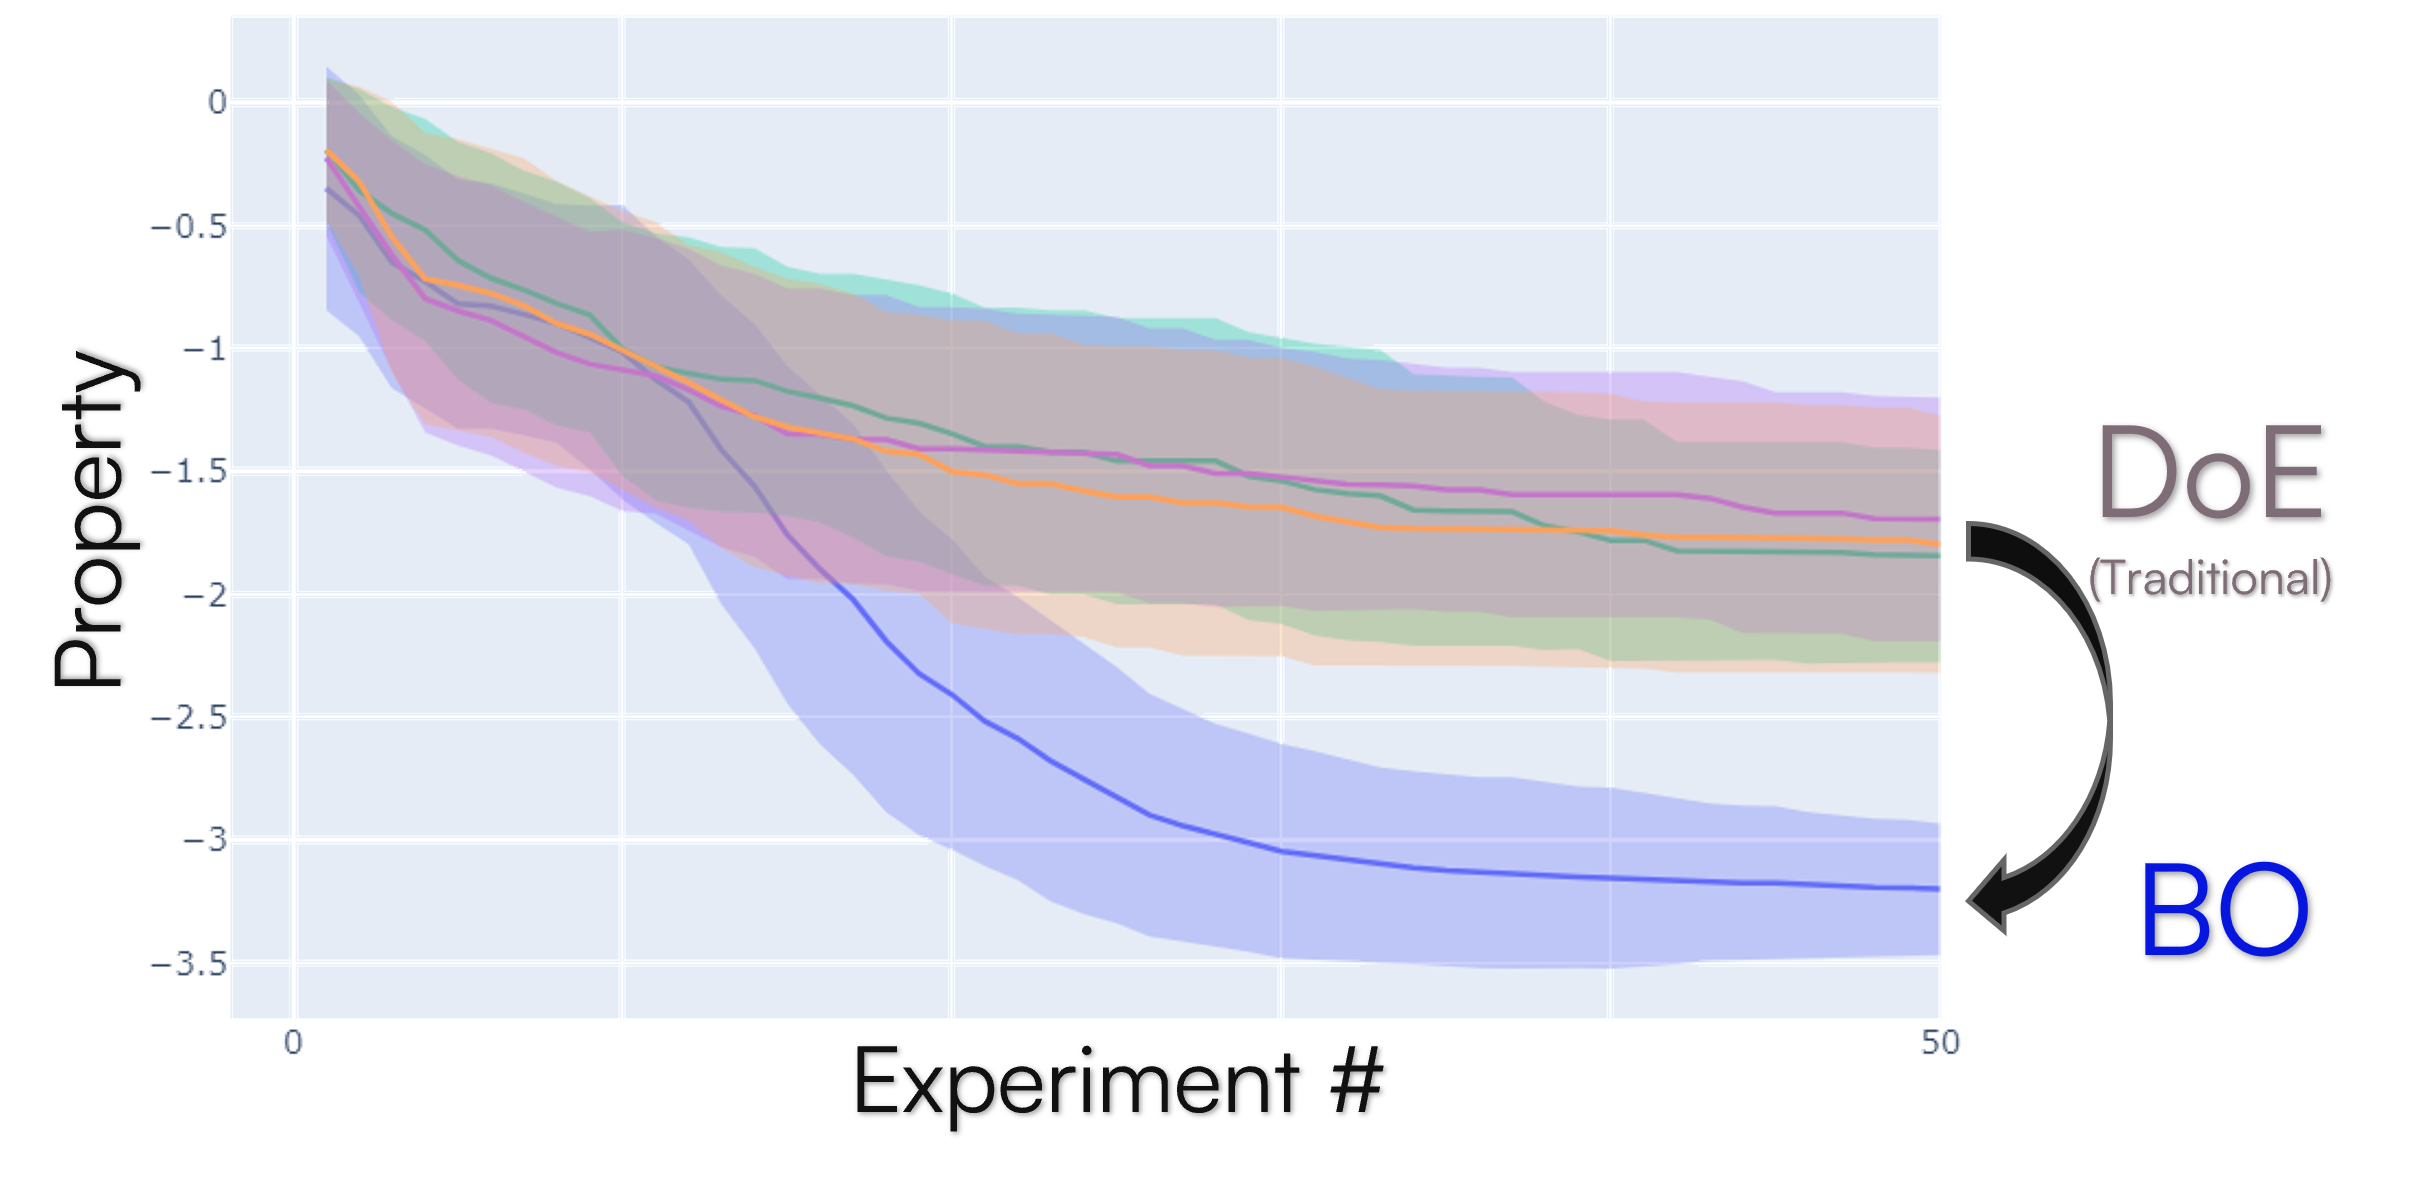
\includegraphics[width=1\linewidth]{latex/figures/intro-bo.png}
    \caption{Optimization traces for traditional design of experiment (DoE) methods compared with \gls{bo}, typically outperforms. \Gls{bo} uses a smart model to predict where to look next in an experiment to find the best results with few experiments.}
    \label{fig:intro-bo}
\end{figure}


\cite{saarLowCostRobotScience2022}

The goal of the AC BO Hackathon was to leverage the expertise of a diverse, global community to advance the development and application of \gls{bo} techniques for solving critical challenges in the physical sciences. The hackathon also aimed to foster collaboration and knowledge sharing among participants from different backgrounds, including academia, national laboratories, government agencies, and private industry. The event attracted 120 active participants from 44 teams, representing 41 academic institutions, 12 national labs, and 9 companies. Likewise, the participants were located in 38 cities, 14 countries, and 4 continents (\cref{fig:map}). A full list of projects, including links to the corresponding GitHub repositories, submission video, and social media post are provided in \cref{tab:projects}.

% \onecolumngrid % (https://tex.stackexchange.com/a/214834/224861)
% % don't remove this linebreak 


\begin{figure*}
    \centering
    % \captionsetup{justification=centering}
    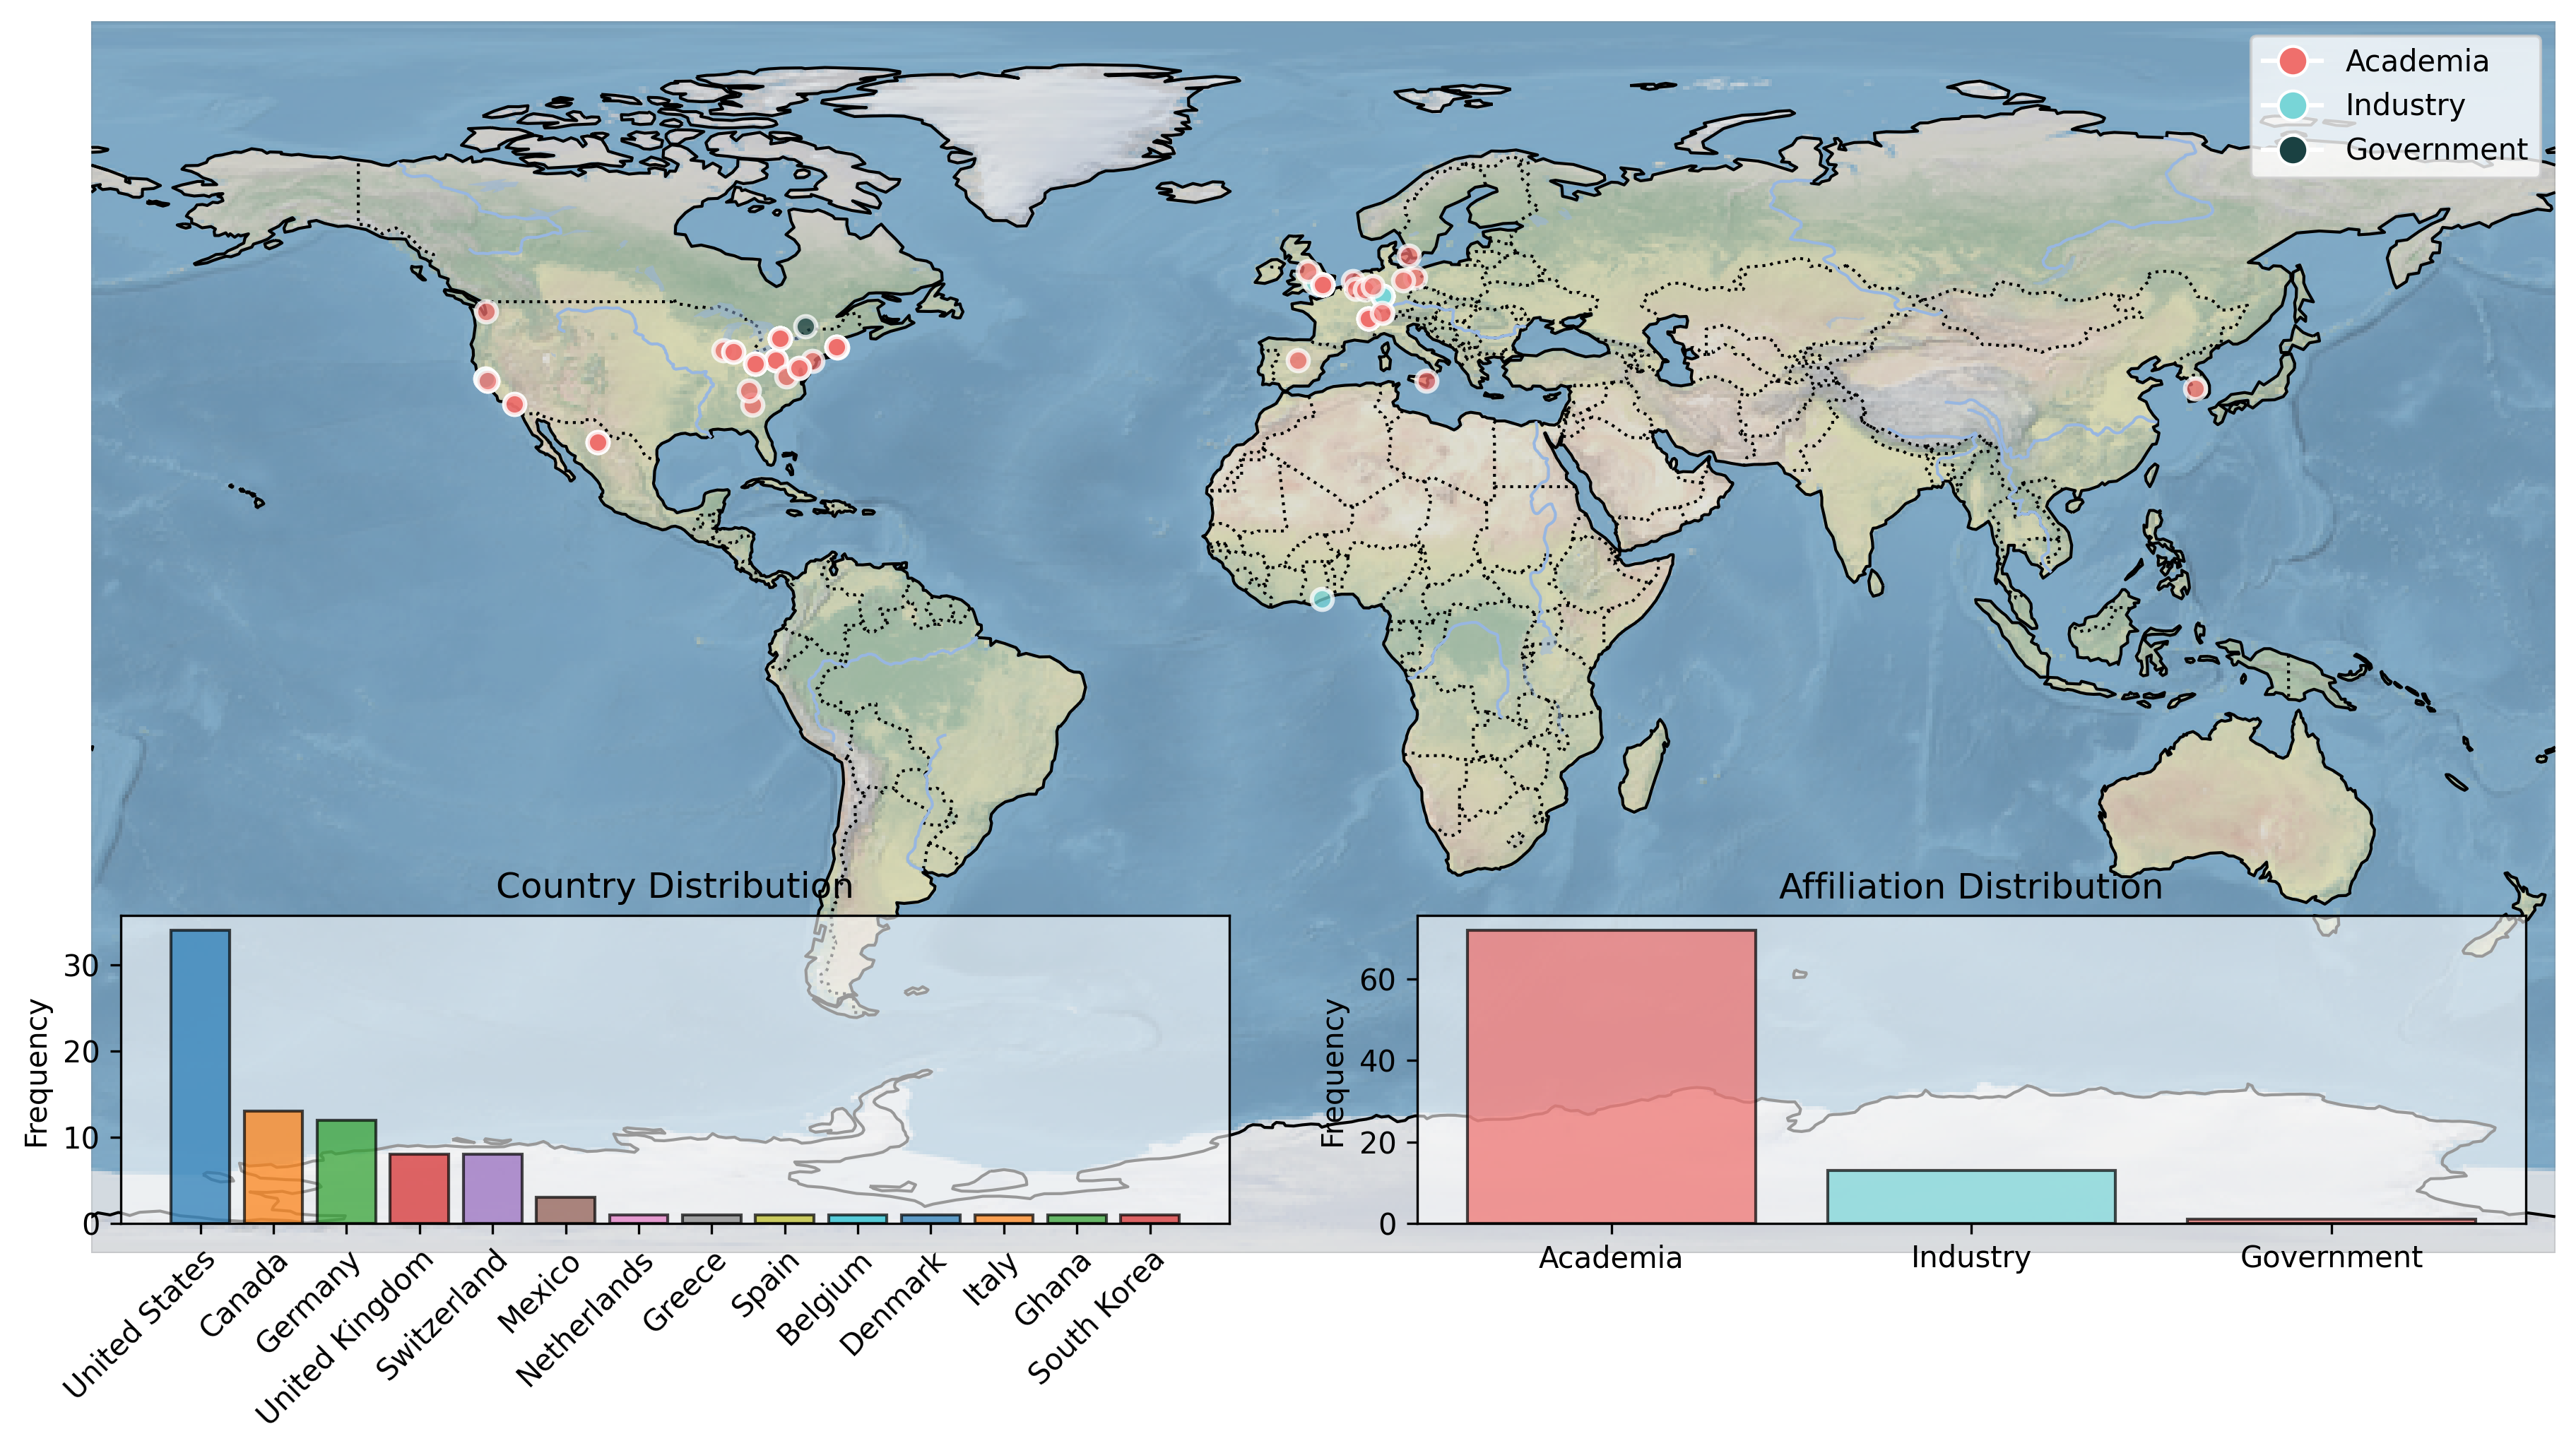
\includegraphics[width=0.95\linewidth]{latex/figures/world_map.png}
    \caption{Demographic distributions of the participating teams and their affiliations. The hackathon supported 129 participants across 60 academic, industry, and government organizations located in 59 cities, 19 countries, and 4 continents. \label{fig:map} }
\end{figure*}




% \begin{table*}[]
% \caption{List of projects and project types, with links to corresponding website project pages, repositories, videos, and social media posts.} \label{tab:projects} \setlength{\extrarowheight}{0.4em} \begin{tabularx}{\textwidth}{>{\centering\arraybackslash}p{1cm} X >{\centering\arraybackslash}X} \toprule \# & Project Name & Links \\ \midrule \href{https://example.com}{\#1} & Project A & \href{https://github.com/example}{\faGithub} \, \href{https://youtube.com}{\faVideo} \, \href{https://twitter.com}{\faTwitter} \tabularnewline \href{https://example.com}{\#2} & Project B & \href{https://github.com/example}{\faGithub} \, \href{https://youtube.com}{\faVideo} \, \href{https://linkedin.com}{\faLinkedin} \tabularnewline \href{https://example.com}{\#3} & Project C & \href{https://github.com/example}{\faGithub} \, \href{https://youtube.com}{\faVideo} \, \href{https://twitter.com}{\faTwitter} \tabularnewline \bottomrule \end{tabularx} 
% \end{table*} 




\section{Hackathon Details and Setup}

Participants were provided with various resources to prepare for the hackathon – this included GitHub classroom assignments with automated feedback, application- and theory-focused videos and tutorials, Python refresher materials, and a list of tools to consider using during the hackathon (\cref{fig:preparation}).

\begin{figure*}
    \centering
    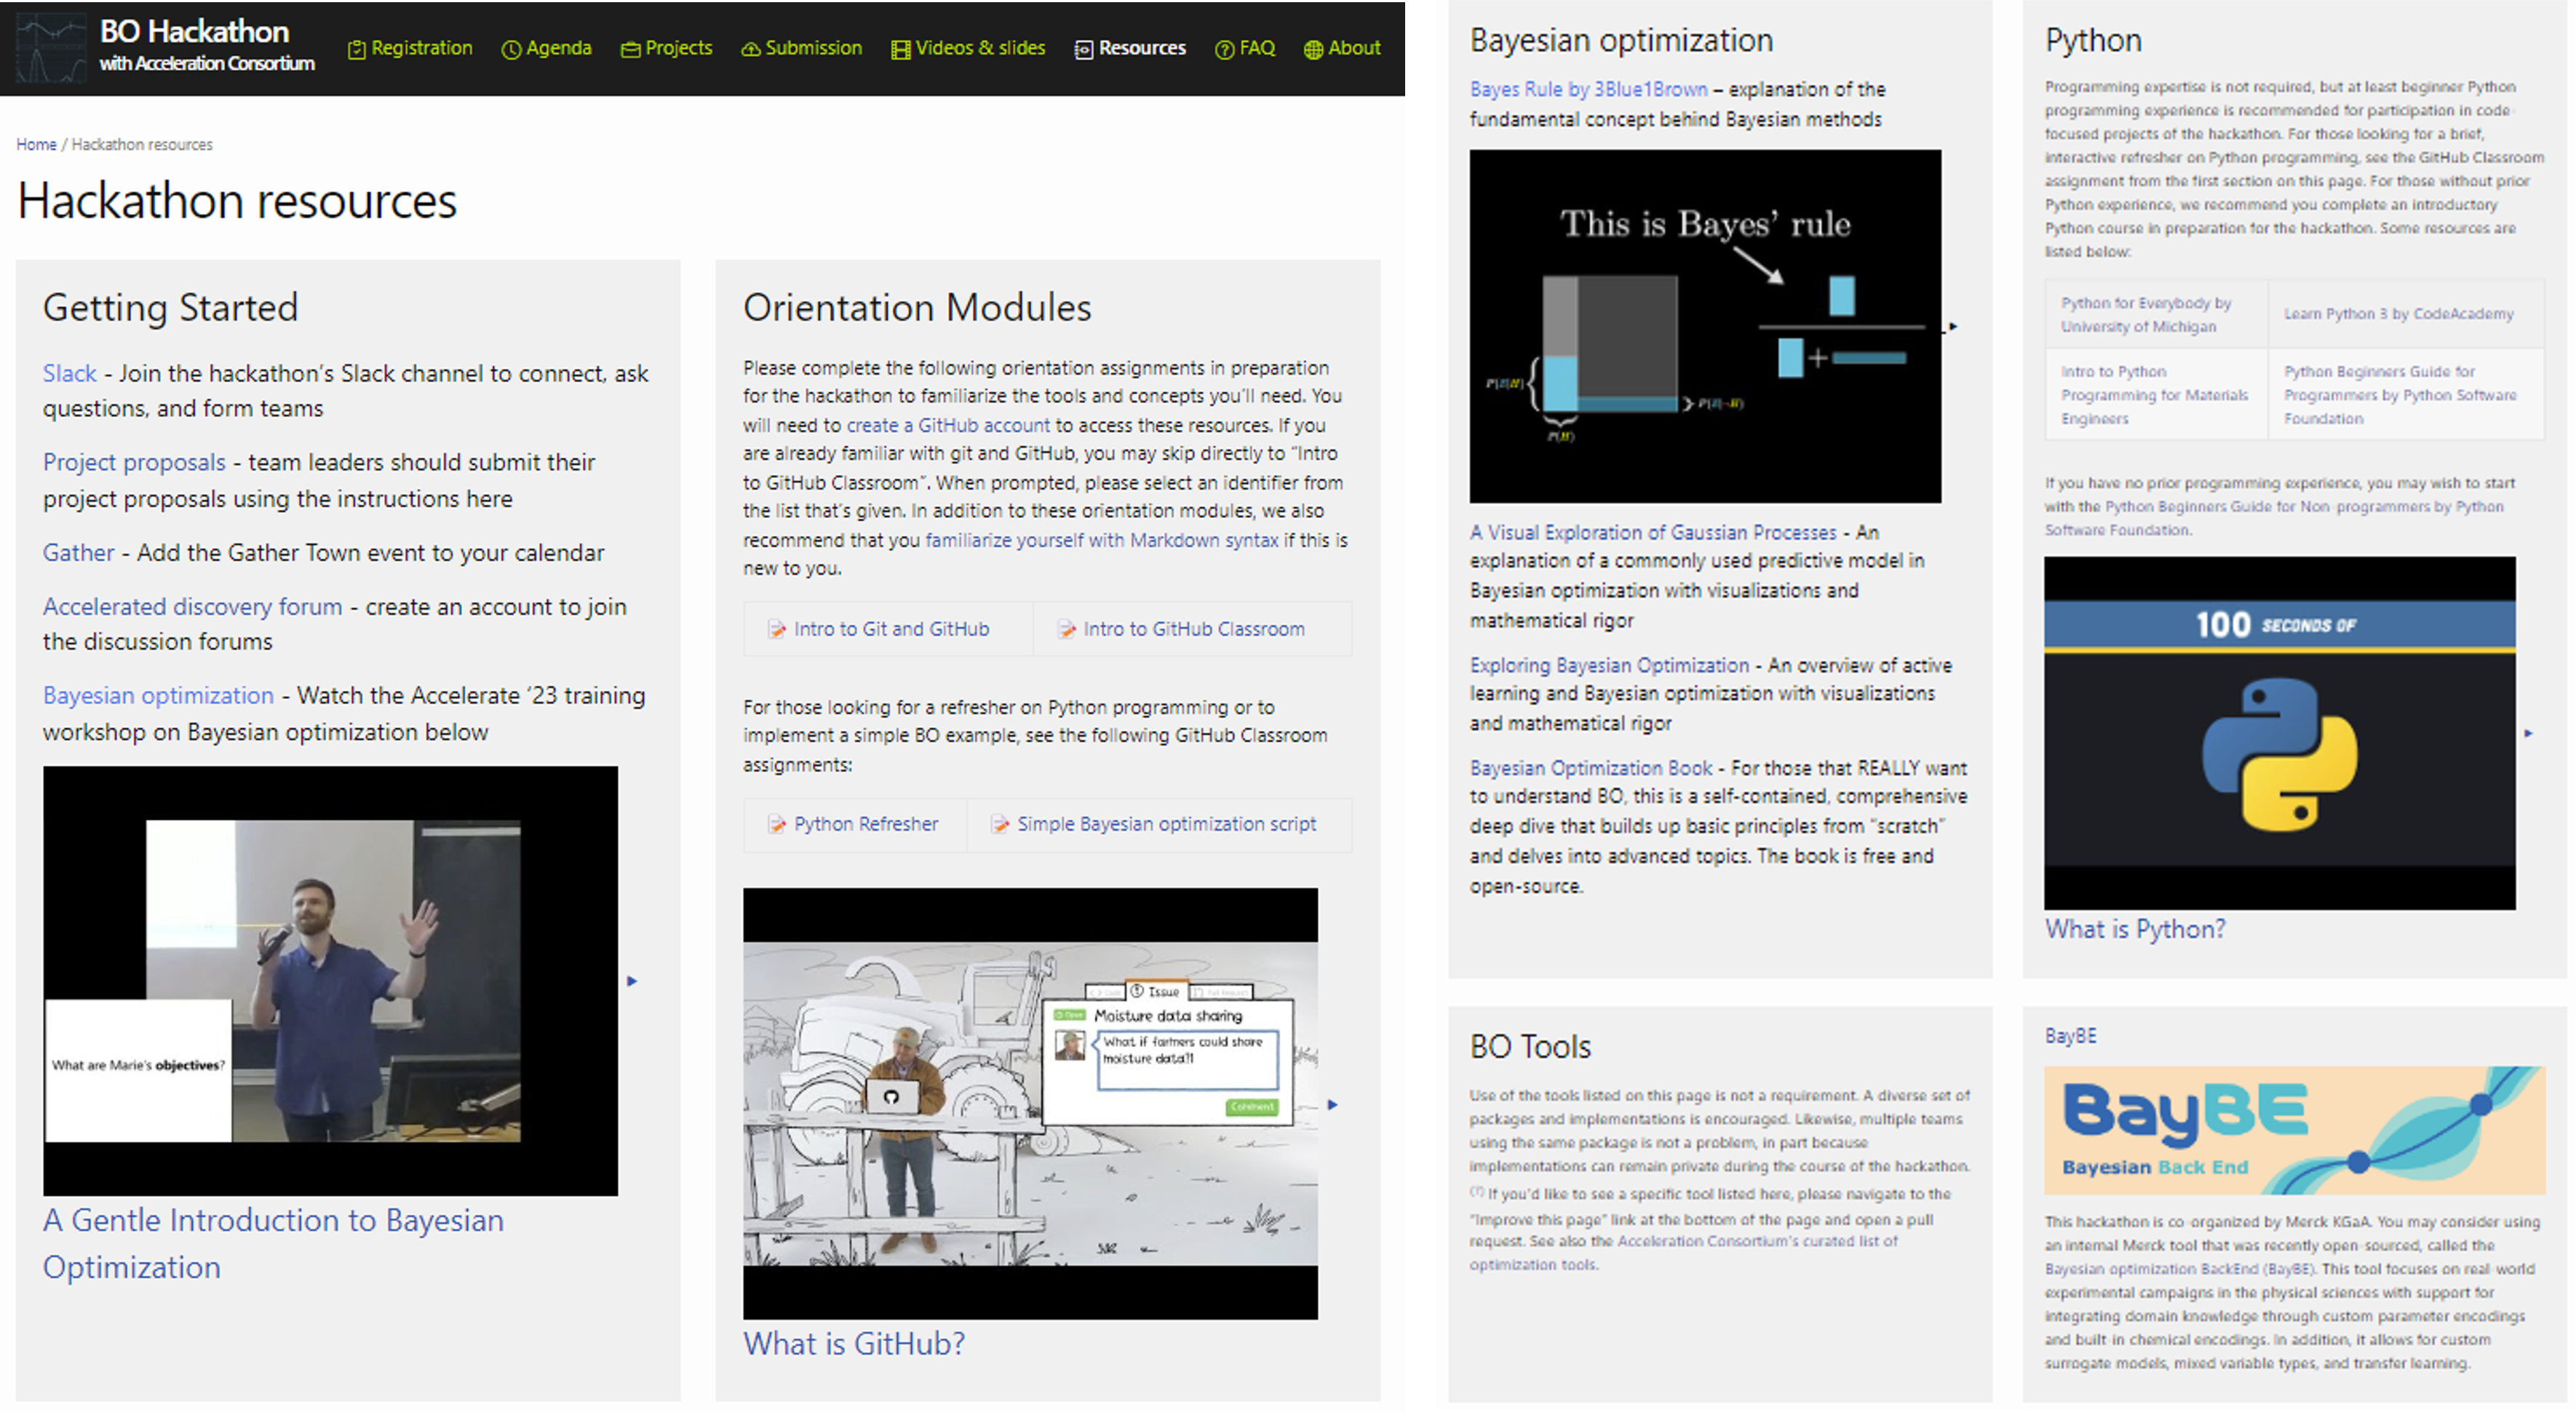
\includegraphics[width=0.98\linewidth]{latex/figures/preparation.png}
    \caption{A snapshot of \href{https://ac-bo-hackathon.github.io/resources/}{resources listed on the hackathon webpage} such as hackathon orientation, intro to \gls{bo}, and a Python refresher assignment. These resources prepared participants to maximize their time during the two-day synchronous portion of the hackathon and helped level the playing field for participants with varied backgrounds and skill levels.}
    \label{fig:preparation}
\end{figure*}

One of the unique aspects of this event is that it was hosted in Gather Town, a sort of union between traditional video conferencing software and retro arcade-style avatars and virtual spaces (\cref{fig:gathertown}). Participants create a custom avatar and maneuver in a two-dimensional space. The videos and audio of other participants appear and become audible when nearby, and fade out when far away, simulating an in-person experience. At the beginning of the hackathon, all participants gathered to listen to keynotes in realtime, which were broadcasted via YouTube live and embedded into the Gather Town space. The videos were then \href{https://ac-bo-hackathon.github.io/videos-slides/}{made available on the hackathon website}, which collectively garnered approximately 1600 views within two months. After the keynotes, teams were assigned tables in breakout rooms, each with a whiteboard. Individual tables were assigned as "private spaces" which isolated the shared audio and video within each space. This had a number of advantages for collaboration within and across teams.

\begin{figure*}
    \centering
    \includegraphics[width=0.95\linewidth]{latex/figures/gathertown.png}
    \caption{Gather town \href{https://ac-bo-hackathon.github.io/videos-slides/}{keynote} room (left), custom avatars (top-right), and an example of a breakout room for teams (bottom-right). Keynotes were broadcasted in realtime to participants via an embedded YouTube livestream. Use of Gather Town helped level the playing field for teams who were in physically separate locations and made it easier for facilitators and other teams to have more natural "check-ins" with other projects.}
    \label{fig:gathertown}
\end{figure*}


The hackathon concluded with a project showcase accompanied by crowdsourced judging within a "poster room" (\cref{fig:poster}).

\begin{figure*}
    \centering
    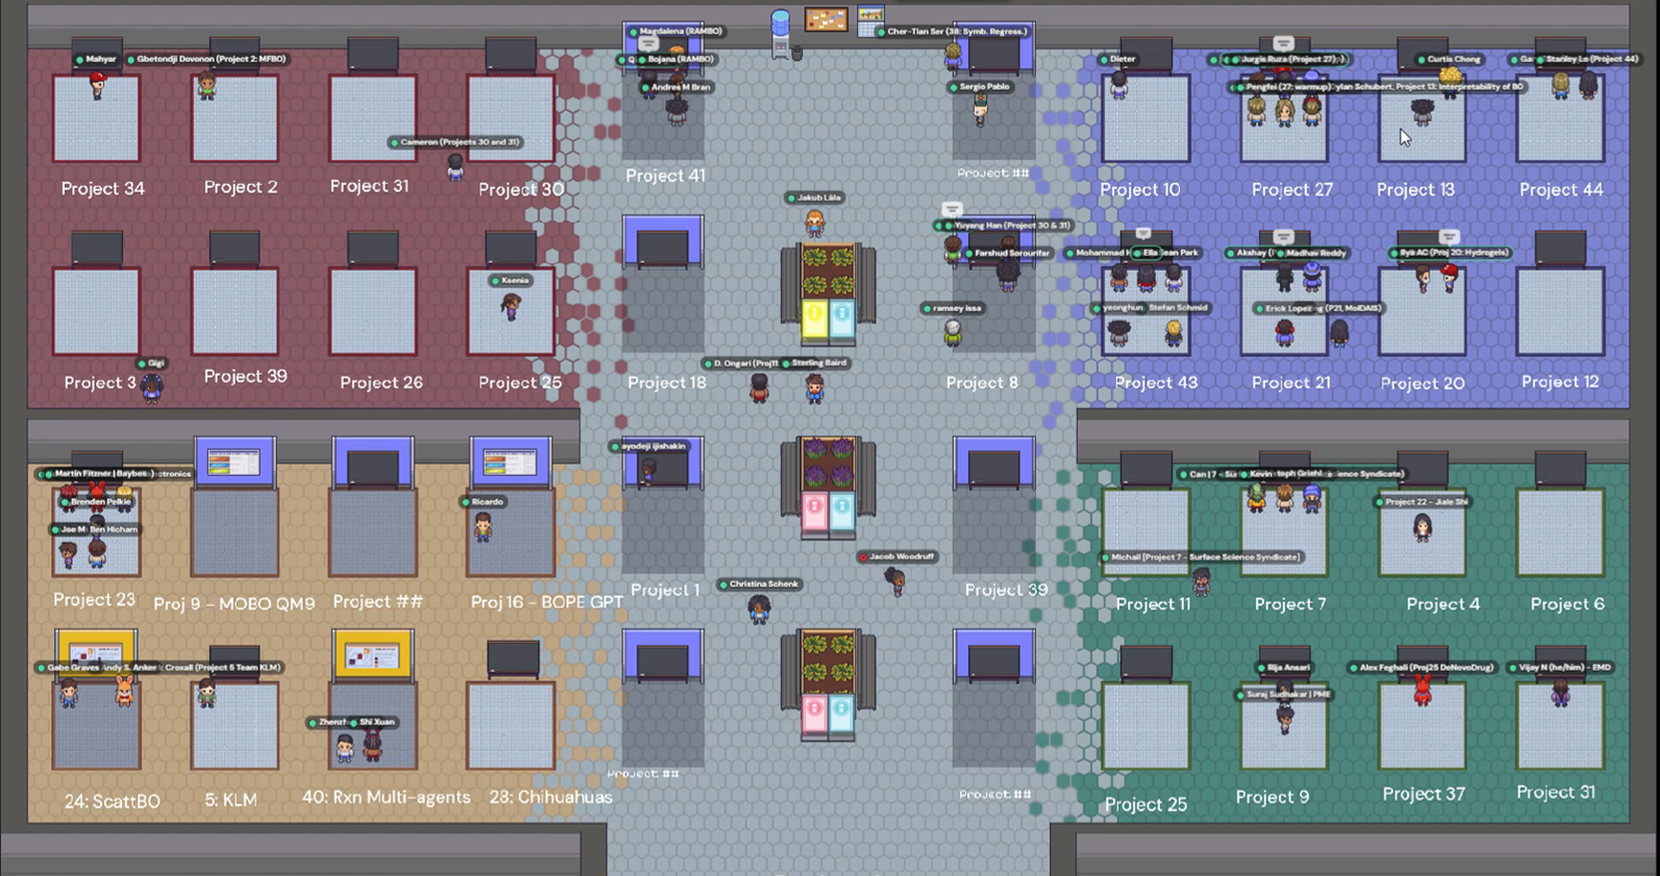
\includegraphics[width=0.95\linewidth]{latex/figures/posters.png}
    \caption{The synchronous portion of the hackathon concluded with a poster session and community judging. One participant noted that "it almost felt like a real poster session."}
    \label{fig:poster}
\end{figure*}

Community judging occurred via \href{https://github.com/anishathalye/gavel}{Gavel}, an automated pairwise comparison judging system. Use of this system helped to improve fairness, scalability, and accuracy by having judges compare projects relative to each other rather than assigning subjective numerical scores (for example, "rate your pain on a scale from 1 to 10, where 10 is the worst possible pain you can imagine"). The approach of pairwise judging reduces bias, allows for handling large competitions efficiently, and produces high-quality rankings using statistical models with dynamic assignments to judges to maximize information gain. It has been successfully used at HackMIT and other events to streamline judging and enhance transparency and credibility.

The corresponding Gavel web app was hosted on Heroku according to directions in the Gavel repository. Individualized links were distributed to judges via email using Gavel's SendGrid integration. Collectively, 35 judges cast 319 votes.



% \clearpage

\begin{longtable*}{>{\centering\arraybackslash}p{1.5cm} @{\hspace{0.4cm}} >{\raggedright\arraybackslash}p{11cm} @{\hspace{1.5cm}} >{\raggedright\arraybackslash}p{2.5cm}}
\caption{List of projects with links to GitHub, Social Media, and Video} \label{tab:projects} \\
% \toprule
% \textbf{Proj. \#} & \textbf{Project Name} & \textbf{Links} \\
% \midrule
% \endfirsthead

\toprule
\textbf{Proj. \#} & \textbf{Project Name} & \textbf{Links} \\
\midrule
\endhead

\midrule \multicolumn{3}{r}{\textit{Continued on the next page}} \\
\midrule
\endfoot

\bottomrule
\endlastfoot

\input{|python3 python_scripts/process_spreadsheet.py}

\end{longtable*}




\begin{table*}[]
\caption{Ranked Projects with Team Names and Prize Distribution. To avoid incentivizing single-person teams and very large teams, both per-person and per-team limits were imposed (e.g., teams of 4 or more would have the max per-team amount divided equally rather than receive the max per-person amount).}
\label{tab:winners}
\setlength{\extrarowheight}{0.8em}
\begin{tabularx}{\textwidth}{>{\centering\arraybackslash}p{1.0cm} >{\centering\arraybackslash}p{1.5cm} >{\centering\arraybackslash}p{3cm} X >{\centering\arraybackslash}p{3cm}}
\toprule
\textbf{Rank} & \textbf{Proj. \#} & \textbf{Team Name} & \textbf{Project Name} & \textbf{Prize* (CAD)} \\ \midrule
1st  & \#23 & Noisy Nerds                & Reliable Surrogate Models of Noisy Data                                                   & 300 (1000 max)          \tabularnewline
2nd  & \#34 & BOMS Prob                  & Streamlining Material Discovery - Bayesian Optimization in Thermal Fluid Mixtures          & 150 (500 max)           \tabularnewline
3rd  & \#7  & Surface Science Syndicate  & BayBE One More Time - Exploring Corrosion Inhibitors for Materials Design                  & 75 (250 max)            \tabularnewline
4th  & \#5  & KLM                        & Comparing Bayesian Optimization Methods \ldots Against Simulated "Human" Decision-making & 40 (125 max)            \tabularnewline
5th  & \#8  & Molecular Representation   & BO for Drug Discovery - What is the role of molecular representation?                      & 40 (125 max)            \tabularnewline
6th  & \#9  & PME No Hikari              & Optimizing The CO2 Adsorption Capacity of Metal-Organic Frameworks Using Thompson Sampling  & 40 (125 max)            \tabularnewline
7th  & \#11 & BlenDS                     & BlendDS - An intuitive specification of the design space for blends of components          & 40 (125 max)            \tabularnewline
8th  & \#30 & SERO Opt                   & Active learning for voltammetry waveform design                                            & 40 (125 max)            \tabularnewline
9th  & \#43 & General Optimizers         & Bayesian Optimization for Generality                                                      & 40 (125 max)            \tabularnewline
10th & \#3  & Sparks Group               & Take Your Time - Measuring Optimization Performance as a Function of ACQF Optimizer Runtime & 40 (125 max)           \tabularnewline
\bottomrule
\end{tabularx}
\end{table*}



% Preparation for the hackathon - 111 GitHub Classroom assignments accepted

% The hackathon was designed with tips, trick, and resources from various sources, such as https://github.com/github/hackathons.


% Hosts: Acceleration Consortium, Merck KGaA



\begin{table*}[]
\caption{Project Topics for the Hackathon. See \href{https://ac-bo-hackathon.github.io/submission/}{the submission page} for more details.}
\label{tab:project_topics}
\setlength{\extrarowheight}{0.4em}
\begin{tabularx}{\textwidth}{>{\centering\arraybackslash}p{0.5cm} p{4.5cm} X}
\toprule
 & \textbf{Topic} & \textbf{Description} \\ \midrule

1 & \textbf{Apply Algorithms} & Choose an algorithm and apply it to a \href{https://huggingface.co/collections/AccelerationConsortium/optimization-benchmarks-66a44daf10de1a0335f28826}{hackathon benchmark task} \\

2 & \textbf{Develop Benchmarks} & Develop a new benchmark and add it to a suite of benchmarks \\

3 & \textbf{Create Tutorials} & Create "gentle introduction" tutorials for \href{https://ac-microcourses.readthedocs.io/en/latest/courses/data-science/overview.html}{advanced optimization topics} \\

4 & \textbf{Propose Tasks} & Propose materials tasks that \textit{can} and \textit{should} be tackled with \gls{bo} \\

5 & \textbf{General} & Other projects related to \gls{bo} for the physical sciences \\

\bottomrule
\end{tabularx}
\end{table*}

% \clearpage

\section{Projects' Key Findings}

This section provides a comprehensive summary and highlights the key findings from all project submissions.
To streamline the evaluation process, all YouTube video submissions were transcribed and analyzed using Anthropics’s \emph{claude-3-5-sonnet-20240620} with a temperature of 0.3, ensuring consistent and accurate processing.
This automated approach enhances efficiency while maintaining a structured and objective assessment of the submissions.


\input{|python3 python_scripts/process_summaries.py}

\clearpage

\section*{Acknowledgements}

\section*{References}

%\printglossaries

% \bibliographystyle{achemso}
\bibliography{latex/references, latex/summaries-ref}

\end{document}